% Options for packages loaded elsewhere
\PassOptionsToPackage{unicode}{hyperref}
\PassOptionsToPackage{hyphens}{url}
%
\documentclass[
]{article}
\title{Class 14 Vaccination Rate Mini Project}
\author{Cindy Tran}
\date{2/13/2022}

\usepackage{amsmath,amssymb}
\usepackage{lmodern}
\usepackage{iftex}
\ifPDFTeX
  \usepackage[T1]{fontenc}
  \usepackage[utf8]{inputenc}
  \usepackage{textcomp} % provide euro and other symbols
\else % if luatex or xetex
  \usepackage{unicode-math}
  \defaultfontfeatures{Scale=MatchLowercase}
  \defaultfontfeatures[\rmfamily]{Ligatures=TeX,Scale=1}
\fi
% Use upquote if available, for straight quotes in verbatim environments
\IfFileExists{upquote.sty}{\usepackage{upquote}}{}
\IfFileExists{microtype.sty}{% use microtype if available
  \usepackage[]{microtype}
  \UseMicrotypeSet[protrusion]{basicmath} % disable protrusion for tt fonts
}{}
\makeatletter
\@ifundefined{KOMAClassName}{% if non-KOMA class
  \IfFileExists{parskip.sty}{%
    \usepackage{parskip}
  }{% else
    \setlength{\parindent}{0pt}
    \setlength{\parskip}{6pt plus 2pt minus 1pt}}
}{% if KOMA class
  \KOMAoptions{parskip=half}}
\makeatother
\usepackage{xcolor}
\IfFileExists{xurl.sty}{\usepackage{xurl}}{} % add URL line breaks if available
\IfFileExists{bookmark.sty}{\usepackage{bookmark}}{\usepackage{hyperref}}
\hypersetup{
  pdftitle={Class 14 Vaccination Rate Mini Project},
  pdfauthor={Cindy Tran},
  hidelinks,
  pdfcreator={LaTeX via pandoc}}
\urlstyle{same} % disable monospaced font for URLs
\usepackage[margin=1in]{geometry}
\usepackage{color}
\usepackage{fancyvrb}
\newcommand{\VerbBar}{|}
\newcommand{\VERB}{\Verb[commandchars=\\\{\}]}
\DefineVerbatimEnvironment{Highlighting}{Verbatim}{commandchars=\\\{\}}
% Add ',fontsize=\small' for more characters per line
\usepackage{framed}
\definecolor{shadecolor}{RGB}{248,248,248}
\newenvironment{Shaded}{\begin{snugshade}}{\end{snugshade}}
\newcommand{\AlertTok}[1]{\textcolor[rgb]{0.94,0.16,0.16}{#1}}
\newcommand{\AnnotationTok}[1]{\textcolor[rgb]{0.56,0.35,0.01}{\textbf{\textit{#1}}}}
\newcommand{\AttributeTok}[1]{\textcolor[rgb]{0.77,0.63,0.00}{#1}}
\newcommand{\BaseNTok}[1]{\textcolor[rgb]{0.00,0.00,0.81}{#1}}
\newcommand{\BuiltInTok}[1]{#1}
\newcommand{\CharTok}[1]{\textcolor[rgb]{0.31,0.60,0.02}{#1}}
\newcommand{\CommentTok}[1]{\textcolor[rgb]{0.56,0.35,0.01}{\textit{#1}}}
\newcommand{\CommentVarTok}[1]{\textcolor[rgb]{0.56,0.35,0.01}{\textbf{\textit{#1}}}}
\newcommand{\ConstantTok}[1]{\textcolor[rgb]{0.00,0.00,0.00}{#1}}
\newcommand{\ControlFlowTok}[1]{\textcolor[rgb]{0.13,0.29,0.53}{\textbf{#1}}}
\newcommand{\DataTypeTok}[1]{\textcolor[rgb]{0.13,0.29,0.53}{#1}}
\newcommand{\DecValTok}[1]{\textcolor[rgb]{0.00,0.00,0.81}{#1}}
\newcommand{\DocumentationTok}[1]{\textcolor[rgb]{0.56,0.35,0.01}{\textbf{\textit{#1}}}}
\newcommand{\ErrorTok}[1]{\textcolor[rgb]{0.64,0.00,0.00}{\textbf{#1}}}
\newcommand{\ExtensionTok}[1]{#1}
\newcommand{\FloatTok}[1]{\textcolor[rgb]{0.00,0.00,0.81}{#1}}
\newcommand{\FunctionTok}[1]{\textcolor[rgb]{0.00,0.00,0.00}{#1}}
\newcommand{\ImportTok}[1]{#1}
\newcommand{\InformationTok}[1]{\textcolor[rgb]{0.56,0.35,0.01}{\textbf{\textit{#1}}}}
\newcommand{\KeywordTok}[1]{\textcolor[rgb]{0.13,0.29,0.53}{\textbf{#1}}}
\newcommand{\NormalTok}[1]{#1}
\newcommand{\OperatorTok}[1]{\textcolor[rgb]{0.81,0.36,0.00}{\textbf{#1}}}
\newcommand{\OtherTok}[1]{\textcolor[rgb]{0.56,0.35,0.01}{#1}}
\newcommand{\PreprocessorTok}[1]{\textcolor[rgb]{0.56,0.35,0.01}{\textit{#1}}}
\newcommand{\RegionMarkerTok}[1]{#1}
\newcommand{\SpecialCharTok}[1]{\textcolor[rgb]{0.00,0.00,0.00}{#1}}
\newcommand{\SpecialStringTok}[1]{\textcolor[rgb]{0.31,0.60,0.02}{#1}}
\newcommand{\StringTok}[1]{\textcolor[rgb]{0.31,0.60,0.02}{#1}}
\newcommand{\VariableTok}[1]{\textcolor[rgb]{0.00,0.00,0.00}{#1}}
\newcommand{\VerbatimStringTok}[1]{\textcolor[rgb]{0.31,0.60,0.02}{#1}}
\newcommand{\WarningTok}[1]{\textcolor[rgb]{0.56,0.35,0.01}{\textbf{\textit{#1}}}}
\usepackage{longtable,booktabs,array}
\usepackage{calc} % for calculating minipage widths
% Correct order of tables after \paragraph or \subparagraph
\usepackage{etoolbox}
\makeatletter
\patchcmd\longtable{\par}{\if@noskipsec\mbox{}\fi\par}{}{}
\makeatother
% Allow footnotes in longtable head/foot
\IfFileExists{footnotehyper.sty}{\usepackage{footnotehyper}}{\usepackage{footnote}}
\makesavenoteenv{longtable}
\usepackage{graphicx}
\makeatletter
\def\maxwidth{\ifdim\Gin@nat@width>\linewidth\linewidth\else\Gin@nat@width\fi}
\def\maxheight{\ifdim\Gin@nat@height>\textheight\textheight\else\Gin@nat@height\fi}
\makeatother
% Scale images if necessary, so that they will not overflow the page
% margins by default, and it is still possible to overwrite the defaults
% using explicit options in \includegraphics[width, height, ...]{}
\setkeys{Gin}{width=\maxwidth,height=\maxheight,keepaspectratio}
% Set default figure placement to htbp
\makeatletter
\def\fps@figure{htbp}
\makeatother
\setlength{\emergencystretch}{3em} % prevent overfull lines
\providecommand{\tightlist}{%
  \setlength{\itemsep}{0pt}\setlength{\parskip}{0pt}}
\setcounter{secnumdepth}{-\maxdimen} % remove section numbering
\ifLuaTeX
  \usepackage{selnolig}  % disable illegal ligatures
\fi

\begin{document}
\maketitle

\hypertarget{getting-started}{%
\section{Getting Started}\label{getting-started}}

\begin{Shaded}
\begin{Highlighting}[]
\CommentTok{\# Import vaccination data}
\NormalTok{vax }\OtherTok{\textless{}{-}} \FunctionTok{read.csv}\NormalTok{(}\StringTok{"covid19vaccinesbyzipcode\_test.csv"}\NormalTok{)}
\FunctionTok{head}\NormalTok{(vax)}
\end{Highlighting}
\end{Shaded}

\begin{verbatim}
##   as_of_date zip_code_tabulation_area local_health_jurisdiction         county
## 1 2021-01-05                    94129             San Francisco  San Francisco
## 2 2021-01-05                    92562                 Riverside      Riverside
## 3 2021-01-05                    92805                    Orange         Orange
## 4 2021-01-05                    92322            San Bernardino San Bernardino
## 5 2021-01-05                    94972                    Sonoma         Sonoma
## 6 2021-01-05                    94107             San Francisco  San Francisco
##   vaccine_equity_metric_quartile                 vem_source
## 1                              4 Healthy Places Index Score
## 2                              3 Healthy Places Index Score
## 3                              1 Healthy Places Index Score
## 4                             NA            No VEM Assigned
## 5                             NA            No VEM Assigned
## 6                              4 Healthy Places Index Score
##   age12_plus_population age5_plus_population persons_fully_vaccinated
## 1                3574.3                 3900                       NA
## 2               53431.1                60184                       12
## 3               61414.4                69071                       25
## 4                 581.0                  632                       NA
## 5                  25.0                   25                       NA
## 6               28946.1                30103                       12
##   persons_partially_vaccinated percent_of_population_fully_vaccinated
## 1                           NA                                     NA
## 2                          868                               0.000199
## 3                          977                               0.000362
## 4                           NA                                     NA
## 5                           NA                                     NA
## 6                          836                               0.000399
##   percent_of_population_partially_vaccinated
## 1                                         NA
## 2                                   0.014422
## 3                                   0.014145
## 4                                         NA
## 5                                         NA
## 6                                   0.027771
##   percent_of_population_with_1_plus_dose booster_recip_count
## 1                                     NA                  NA
## 2                               0.014621                  NA
## 3                               0.014507                  NA
## 4                                     NA                  NA
## 5                                     NA                  NA
## 6                               0.028170                  NA
##                                                                redacted
## 1 Information redacted in accordance with CA state privacy requirements
## 2 Information redacted in accordance with CA state privacy requirements
## 3 Information redacted in accordance with CA state privacy requirements
## 4 Information redacted in accordance with CA state privacy requirements
## 5 Information redacted in accordance with CA state privacy requirements
## 6 Information redacted in accordance with CA state privacy requirements
\end{verbatim}

\begin{quote}
Q1. What column details the total number of people fully vaccinated?
\end{quote}

persons\_fully\_vaccinated

\begin{quote}
Q2. What column details the Zip code tabulation area?
\end{quote}

zip\_code\_tabulation\_area

\begin{quote}
Q3. What is the earliest date in this dataset?
\end{quote}

2021-01-05

\begin{quote}
Q4. What is the latest date in this dataset?
\end{quote}

2022-02-08

\begin{Shaded}
\begin{Highlighting}[]
\CommentTok{\#install.packages("skimr")}
\FunctionTok{library}\NormalTok{(skimr)}
\NormalTok{skimr}\SpecialCharTok{::}\FunctionTok{skim}\NormalTok{(vax)}
\end{Highlighting}
\end{Shaded}

\begin{longtable}[]{@{}ll@{}}
\caption{Data summary}\tabularnewline
\toprule
\endhead
Name & vax \\
Number of rows & 102312 \\
Number of columns & 15 \\
\_\_\_\_\_\_\_\_\_\_\_\_\_\_\_\_\_\_\_\_\_\_\_ & \\
Column type frequency: & \\
character & 5 \\
numeric & 10 \\
\_\_\_\_\_\_\_\_\_\_\_\_\_\_\_\_\_\_\_\_\_\_\_\_ & \\
Group variables & None \\
\bottomrule
\end{longtable}

\textbf{Variable type: character}

\begin{longtable}[]{@{}lrrrrrrr@{}}
\toprule
skim\_variable & n\_missing & complete\_rate & min & max & empty &
n\_unique & whitespace \\
\midrule
\endhead
as\_of\_date & 0 & 1 & 10 & 10 & 0 & 58 & 0 \\
local\_health\_jurisdiction & 0 & 1 & 0 & 15 & 290 & 62 & 0 \\
county & 0 & 1 & 0 & 15 & 290 & 59 & 0 \\
vem\_source & 0 & 1 & 15 & 26 & 0 & 3 & 0 \\
redacted & 0 & 1 & 2 & 69 & 0 & 2 & 0 \\
\bottomrule
\end{longtable}

\textbf{Variable type: numeric}

\begin{longtable}[]{@{}
  >{\raggedright\arraybackslash}p{(\columnwidth - 20\tabcolsep) * \real{0.26}}
  >{\raggedleft\arraybackslash}p{(\columnwidth - 20\tabcolsep) * \real{0.06}}
  >{\raggedleft\arraybackslash}p{(\columnwidth - 20\tabcolsep) * \real{0.08}}
  >{\raggedleft\arraybackslash}p{(\columnwidth - 20\tabcolsep) * \real{0.05}}
  >{\raggedleft\arraybackslash}p{(\columnwidth - 20\tabcolsep) * \real{0.05}}
  >{\raggedleft\arraybackslash}p{(\columnwidth - 20\tabcolsep) * \real{0.04}}
  >{\raggedleft\arraybackslash}p{(\columnwidth - 20\tabcolsep) * \real{0.05}}
  >{\raggedleft\arraybackslash}p{(\columnwidth - 20\tabcolsep) * \real{0.05}}
  >{\raggedleft\arraybackslash}p{(\columnwidth - 20\tabcolsep) * \real{0.05}}
  >{\raggedleft\arraybackslash}p{(\columnwidth - 20\tabcolsep) * \real{0.05}}
  >{\raggedright\arraybackslash}p{(\columnwidth - 20\tabcolsep) * \real{0.24}}@{}}
\toprule
\begin{minipage}[b]{\linewidth}\raggedright
skim\_variable
\end{minipage} & \begin{minipage}[b]{\linewidth}\raggedleft
n\_missing
\end{minipage} & \begin{minipage}[b]{\linewidth}\raggedleft
complete\_rate
\end{minipage} & \begin{minipage}[b]{\linewidth}\raggedleft
mean
\end{minipage} & \begin{minipage}[b]{\linewidth}\raggedleft
sd
\end{minipage} & \begin{minipage}[b]{\linewidth}\raggedleft
p0
\end{minipage} & \begin{minipage}[b]{\linewidth}\raggedleft
p25
\end{minipage} & \begin{minipage}[b]{\linewidth}\raggedleft
p50
\end{minipage} & \begin{minipage}[b]{\linewidth}\raggedleft
p75
\end{minipage} & \begin{minipage}[b]{\linewidth}\raggedleft
p100
\end{minipage} & \begin{minipage}[b]{\linewidth}\raggedright
hist
\end{minipage} \\
\midrule
\endhead
zip\_code\_tabulation\_area & 0 & 1.00 & 93665.11 & 1817.39 & 90001 &
92257.75 & 93658.50 & 95380.50 & 97635.0 & ▃▅▅▇▁ \\
vaccine\_equity\_metric\_quartile & 5046 & 0.95 & 2.44 & 1.11 & 1 & 1.00
& 2.00 & 3.00 & 4.0 & ▇▇▁▇▇ \\
age12\_plus\_population & 0 & 1.00 & 18895.04 & 18993.92 & 0 & 1346.95 &
13685.10 & 31756.12 & 88556.7 & ▇▃▂▁▁ \\
age5\_plus\_population & 0 & 1.00 & 20875.24 & 21106.02 & 0 & 1460.50 &
15364.00 & 34877.00 & 101902.0 & ▇▃▂▁▁ \\
persons\_fully\_vaccinated & 9640 & 0.91 & 10890.58 & 12771.81 & 11 &
623.00 & 5313.00 & 18338.00 & 85970.0 & ▇▂▁▁▁ \\
persons\_partially\_vaccinated & 9640 & 0.91 & 1845.39 & 2062.93 & 11 &
189.00 & 1251.00 & 2790.00 & 29153.0 & ▇▁▁▁▁ \\
percent\_of\_population\_fully\_vaccinated & 9640 & 0.91 & 0.48 & 0.27 &
0 & 0.27 & 0.51 & 0.69 & 1.0 & ▆▅▇▇▃ \\
percent\_of\_population\_partially\_vaccinated & 9640 & 0.91 & 0.09 &
0.11 & 0 & 0.06 & 0.07 & 0.10 & 1.0 & ▇▁▁▁▁ \\
percent\_of\_population\_with\_1\_plus\_dose & 9640 & 0.91 & 0.56 & 0.27
& 0 & 0.37 & 0.59 & 0.76 & 1.0 & ▃▃▆▇▅ \\
booster\_recip\_count & 63642 & 0.38 & 3516.20 & 5246.71 & 11 & 150.00 &
908.00 & 5069.75 & 48283.0 & ▇▁▁▁▁ \\
\bottomrule
\end{longtable}

\begin{quote}
Q5. How many numeric columns are in this dataset?
\end{quote}

15

\begin{quote}
Q6. Note that there are ``missing values'' in the dataset. How many NA
values there in the persons\_fully\_vaccinated column?
\end{quote}

\begin{Shaded}
\begin{Highlighting}[]
\FunctionTok{sum}\NormalTok{( }\FunctionTok{is.na}\NormalTok{(vax}\SpecialCharTok{$}\NormalTok{persons\_fully\_vaccinated) )}
\end{Highlighting}
\end{Shaded}

\begin{verbatim}
## [1] 9640
\end{verbatim}

9640

\begin{quote}
Q7. What percent of persons\_fully\_vaccinated values are missing (to 2
significant figures)?
\end{quote}

\begin{Shaded}
\begin{Highlighting}[]
\DecValTok{9640} \SpecialCharTok{/}\NormalTok{ (}\FunctionTok{sum}\NormalTok{(}\SpecialCharTok{!}\FunctionTok{is.na}\NormalTok{(vax}\SpecialCharTok{$}\NormalTok{persons\_fully\_vaccinated))) }\SpecialCharTok{*} \DecValTok{100}
\end{Highlighting}
\end{Shaded}

\begin{verbatim}
## [1] 10.40228
\end{verbatim}

10\%

\begin{quote}
Q8. {[}Optional{]}: Why might this data be missing?
\end{quote}

This data is posisbly missing because some counties did not have collect
this information.

\hypertarget{working-with-dates}{%
\subsection{Working with Dates}\label{working-with-dates}}

\begin{Shaded}
\begin{Highlighting}[]
\FunctionTok{library}\NormalTok{(lubridate)}
\end{Highlighting}
\end{Shaded}

\begin{verbatim}
## 
## Attaching package: 'lubridate'
\end{verbatim}

\begin{verbatim}
## The following objects are masked from 'package:base':
## 
##     date, intersect, setdiff, union
\end{verbatim}

\begin{Shaded}
\begin{Highlighting}[]
\FunctionTok{today}\NormalTok{()}
\end{Highlighting}
\end{Shaded}

\begin{verbatim}
## [1] "2022-02-14"
\end{verbatim}

\begin{Shaded}
\begin{Highlighting}[]
\CommentTok{\# Specify that we are using the Year{-}month{-}day format}
\NormalTok{vax}\SpecialCharTok{$}\NormalTok{as\_of\_date }\OtherTok{\textless{}{-}} \FunctionTok{ymd}\NormalTok{(vax}\SpecialCharTok{$}\NormalTok{as\_of\_date)}
\end{Highlighting}
\end{Shaded}

Now we can do math with dates. For example: How many days have passed
since the first vaccination reported in this dataset?

\begin{Shaded}
\begin{Highlighting}[]
\FunctionTok{today}\NormalTok{() }\SpecialCharTok{{-}}\NormalTok{ vax}\SpecialCharTok{$}\NormalTok{as\_of\_date[}\DecValTok{1}\NormalTok{]}
\end{Highlighting}
\end{Shaded}

\begin{verbatim}
## Time difference of 405 days
\end{verbatim}

Using the last and the first date value we can now determine how many
days the dataset span.

\begin{Shaded}
\begin{Highlighting}[]
\NormalTok{vax}\SpecialCharTok{$}\NormalTok{as\_of\_date[}\FunctionTok{nrow}\NormalTok{(vax)] }\SpecialCharTok{{-}}\NormalTok{ vax}\SpecialCharTok{$}\NormalTok{as\_of\_date[}\DecValTok{1}\NormalTok{]}
\end{Highlighting}
\end{Shaded}

\begin{verbatim}
## Time difference of 399 days
\end{verbatim}

\begin{quote}
Q9. How many days have passed since the last update of the dataset?
\end{quote}

\begin{Shaded}
\begin{Highlighting}[]
\FunctionTok{today}\NormalTok{() }\SpecialCharTok{{-}}\NormalTok{ vax}\SpecialCharTok{$}\NormalTok{as\_of\_date[}\FunctionTok{nrow}\NormalTok{(vax)]}
\end{Highlighting}
\end{Shaded}

\begin{verbatim}
## Time difference of 6 days
\end{verbatim}

\begin{quote}
Q10. How many unique dates are in the dataset (i.e.~how many different
dates are detailed)?
\end{quote}

\begin{Shaded}
\begin{Highlighting}[]
\FunctionTok{length}\NormalTok{(}\FunctionTok{unique}\NormalTok{(vax}\SpecialCharTok{$}\NormalTok{as\_of\_date))}
\end{Highlighting}
\end{Shaded}

\begin{verbatim}
## [1] 58
\end{verbatim}

\hypertarget{working-with-zip-codes}{%
\section{Working with ZIP Codes}\label{working-with-zip-codes}}

\begin{Shaded}
\begin{Highlighting}[]
\CommentTok{\#install.packages("zipcodeR")}
\FunctionTok{library}\NormalTok{(zipcodeR)}
\end{Highlighting}
\end{Shaded}

Find the centroid of the La Jolla 92037 (i.e.~UC San Diego) ZIP code
area.

\begin{Shaded}
\begin{Highlighting}[]
\FunctionTok{geocode\_zip}\NormalTok{(}\StringTok{\textquotesingle{}92037\textquotesingle{}}\NormalTok{)}
\end{Highlighting}
\end{Shaded}

\begin{verbatim}
## # A tibble: 1 x 3
##   zipcode   lat   lng
##   <chr>   <dbl> <dbl>
## 1 92037    32.8 -117.
\end{verbatim}

Calculate the distance between the centroids of any two ZIP codes in
miles

\begin{Shaded}
\begin{Highlighting}[]
\FunctionTok{zip\_distance}\NormalTok{(}\StringTok{\textquotesingle{}92037\textquotesingle{}}\NormalTok{,}\StringTok{\textquotesingle{}92109\textquotesingle{}}\NormalTok{)}
\end{Highlighting}
\end{Shaded}

\begin{verbatim}
##   zipcode_a zipcode_b distance
## 1     92037     92109     2.33
\end{verbatim}

We can pull census data about ZIP code areas (including median household
income etc.

\begin{Shaded}
\begin{Highlighting}[]
\FunctionTok{reverse\_zipcode}\NormalTok{(}\FunctionTok{c}\NormalTok{(}\StringTok{\textquotesingle{}92037\textquotesingle{}}\NormalTok{, }\StringTok{"92109"}\NormalTok{) )}
\end{Highlighting}
\end{Shaded}

\begin{verbatim}
## # A tibble: 2 x 24
##   zipcode zipcode_type major_city post_office_city common_city_list county state
##   <chr>   <chr>        <chr>      <chr>                      <blob> <chr>  <chr>
## 1 92037   Standard     La Jolla   La Jolla, CA           <raw 20 B> San D~ CA   
## 2 92109   Standard     San Diego  San Diego, CA          <raw 21 B> San D~ CA   
## # ... with 17 more variables: lat <dbl>, lng <dbl>, timezone <chr>,
## #   radius_in_miles <dbl>, area_code_list <blob>, population <int>,
## #   population_density <dbl>, land_area_in_sqmi <dbl>,
## #   water_area_in_sqmi <dbl>, housing_units <int>,
## #   occupied_housing_units <int>, median_home_value <int>,
## #   median_household_income <int>, bounds_west <dbl>, bounds_east <dbl>,
## #   bounds_north <dbl>, bounds_south <dbl>
\end{verbatim}

\begin{Shaded}
\begin{Highlighting}[]
\CommentTok{\# Pull data for all ZIP codes in the dataset}
\NormalTok{zipdata }\OtherTok{\textless{}{-}} \FunctionTok{reverse\_zipcode}\NormalTok{( vax}\SpecialCharTok{$}\NormalTok{zip\_code\_tabulation\_area )}
\end{Highlighting}
\end{Shaded}

\hypertarget{focus-on-the-san-diego-area}{%
\section{Focus on the San Diego
Area}\label{focus-on-the-san-diego-area}}

\begin{Shaded}
\begin{Highlighting}[]
\CommentTok{\# Subset to San Diego county only areas}
\NormalTok{sd }\OtherTok{\textless{}{-}}\NormalTok{ vax[ vax}\SpecialCharTok{$}\NormalTok{county }\SpecialCharTok{==} \StringTok{"San Diego"}\NormalTok{ , ]}
\FunctionTok{nrow}\NormalTok{(sd)}
\end{Highlighting}
\end{Shaded}

\begin{verbatim}
## [1] 6206
\end{verbatim}

\begin{Shaded}
\begin{Highlighting}[]
\FunctionTok{library}\NormalTok{(dplyr)}
\end{Highlighting}
\end{Shaded}

\begin{verbatim}
## 
## Attaching package: 'dplyr'
\end{verbatim}

\begin{verbatim}
## The following objects are masked from 'package:stats':
## 
##     filter, lag
\end{verbatim}

\begin{verbatim}
## The following objects are masked from 'package:base':
## 
##     intersect, setdiff, setequal, union
\end{verbatim}

\begin{Shaded}
\begin{Highlighting}[]
\NormalTok{sd }\OtherTok{\textless{}{-}} \FunctionTok{filter}\NormalTok{(vax, county }\SpecialCharTok{==} \StringTok{"San Diego"}\NormalTok{)}
\FunctionTok{nrow}\NormalTok{(sd)}
\end{Highlighting}
\end{Shaded}

\begin{verbatim}
## [1] 6206
\end{verbatim}

Using dplyr is often more convenient when we are subsetting across
multiple criteria - for example all San Diego county areas with a
population of over 10,000.

\begin{Shaded}
\begin{Highlighting}[]
\NormalTok{sd}\FloatTok{.10} \OtherTok{\textless{}{-}} \FunctionTok{filter}\NormalTok{(vax, county }\SpecialCharTok{==} \StringTok{"San Diego"} \SpecialCharTok{\&}
\NormalTok{                age5\_plus\_population }\SpecialCharTok{\textgreater{}} \DecValTok{10000}\NormalTok{)}
\end{Highlighting}
\end{Shaded}

\begin{quote}
Q11. How many distinct zip codes are listed for San Diego County?
\end{quote}

\begin{Shaded}
\begin{Highlighting}[]
\FunctionTok{length}\NormalTok{(}\FunctionTok{unique}\NormalTok{(sd}\SpecialCharTok{$}\NormalTok{zip\_code\_tabulation\_area))}
\end{Highlighting}
\end{Shaded}

\begin{verbatim}
## [1] 107
\end{verbatim}

\begin{quote}
Q12. What San Diego County Zip code area has the largest 12 + Population
in this dataset?
\end{quote}

\begin{Shaded}
\begin{Highlighting}[]
\FunctionTok{which.max}\NormalTok{(sd}\SpecialCharTok{$}\NormalTok{age12\_plus\_population)}
\end{Highlighting}
\end{Shaded}

\begin{verbatim}
## [1] 56
\end{verbatim}

\begin{Shaded}
\begin{Highlighting}[]
\NormalTok{sd[}\DecValTok{56}\NormalTok{,]}
\end{Highlighting}
\end{Shaded}

\begin{verbatim}
##    as_of_date zip_code_tabulation_area local_health_jurisdiction    county
## 56 2021-01-05                    92154                 San Diego San Diego
##    vaccine_equity_metric_quartile                 vem_source
## 56                              2 Healthy Places Index Score
##    age12_plus_population age5_plus_population persons_fully_vaccinated
## 56               76365.2                82971                       33
##    persons_partially_vaccinated percent_of_population_fully_vaccinated
## 56                         1357                               0.000398
##    percent_of_population_partially_vaccinated
## 56                                   0.016355
##    percent_of_population_with_1_plus_dose booster_recip_count
## 56                               0.016753                  NA
##                                                                 redacted
## 56 Information redacted in accordance with CA state privacy requirements
\end{verbatim}

92154

\begin{quote}
Q13. What is the overall average ``Percent of Population Fully
Vaccinated'' value for all San Diego ``County'' as of ``2021-11-09''?
\end{quote}

\begin{Shaded}
\begin{Highlighting}[]
\NormalTok{q13 }\OtherTok{\textless{}{-}} \FunctionTok{filter}\NormalTok{ (sd, as\_of\_date }\SpecialCharTok{==} \StringTok{"2021{-}11{-}09"}\NormalTok{)}
\FunctionTok{mean}\NormalTok{(q13}\SpecialCharTok{$}\NormalTok{percent\_of\_population\_fully\_vaccinated, }\AttributeTok{na.rm =} \ConstantTok{TRUE}\NormalTok{)}
\end{Highlighting}
\end{Shaded}

\begin{verbatim}
## [1] 0.6961169
\end{verbatim}

\begin{quote}
Q14. Using either ggplot or base R graphics make a summary figure that
shows the distribution of Percent of Population Fully Vaccinated values
as of ``2021-11-09''?
\end{quote}

\begin{Shaded}
\begin{Highlighting}[]
\FunctionTok{library}\NormalTok{(ggplot2)}
\FunctionTok{ggplot}\NormalTok{(q13) }\SpecialCharTok{+}
  \FunctionTok{aes}\NormalTok{(}\AttributeTok{x =}\NormalTok{ percent\_of\_population\_fully\_vaccinated) }\SpecialCharTok{+} 
  \FunctionTok{geom\_histogram}\NormalTok{()}
\end{Highlighting}
\end{Shaded}

\begin{verbatim}
## `stat_bin()` using `bins = 30`. Pick better value with `binwidth`.
\end{verbatim}

\begin{verbatim}
## Warning: Removed 4 rows containing non-finite values (stat_bin).
\end{verbatim}

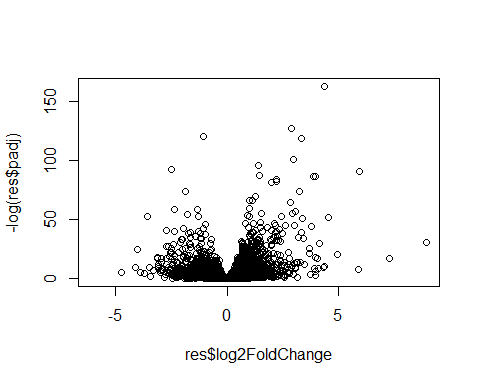
\includegraphics{class14lab_files/figure-latex/unnamed-chunk-22-1.pdf}

\hypertarget{focus-on-ucsdla-jolla}{%
\subsection{Focus on UCSD/La Jolla}\label{focus-on-ucsdla-jolla}}

\begin{Shaded}
\begin{Highlighting}[]
\NormalTok{ucsd }\OtherTok{\textless{}{-}} \FunctionTok{filter}\NormalTok{(sd, zip\_code\_tabulation\_area}\SpecialCharTok{==}\StringTok{"92037"}\NormalTok{)}
\NormalTok{ucsd[}\DecValTok{1}\NormalTok{,]}\SpecialCharTok{$}\NormalTok{age5\_plus\_population}
\end{Highlighting}
\end{Shaded}

\begin{verbatim}
## [1] 36144
\end{verbatim}

\begin{quote}
Q15. Using ggplot make a graph of the vaccination rate time course for
the 92037 ZIP code area:
\end{quote}

\begin{Shaded}
\begin{Highlighting}[]
\FunctionTok{ggplot}\NormalTok{(ucsd) }\SpecialCharTok{+}
  \FunctionTok{aes}\NormalTok{(as\_of\_date, percent\_of\_population\_fully\_vaccinated) }\SpecialCharTok{+}
  \FunctionTok{geom\_point}\NormalTok{() }\SpecialCharTok{+}
  \FunctionTok{geom\_line}\NormalTok{(}\AttributeTok{group=}\DecValTok{1}\NormalTok{) }\SpecialCharTok{+}
  \FunctionTok{ylim}\NormalTok{(}\FunctionTok{c}\NormalTok{(}\DecValTok{0}\NormalTok{,}\DecValTok{1}\NormalTok{)) }\SpecialCharTok{+}
  \FunctionTok{labs}\NormalTok{(}\AttributeTok{x=}\StringTok{"Date"}\NormalTok{, }\AttributeTok{y=}\StringTok{"Percent Vaccinated"}\NormalTok{)}
\end{Highlighting}
\end{Shaded}

\includegraphics{class14lab_files/figure-latex/unnamed-chunk-24-1.pdf}

\hypertarget{comparing-92037-to-other-similarly-sized-areas}{%
\subsection{Comparing 92037 to Other SImilarly Sized
Areas}\label{comparing-92037-to-other-similarly-sized-areas}}

\begin{Shaded}
\begin{Highlighting}[]
\CommentTok{\# Subset to all CA areas with a population as large as 92037}
\NormalTok{vax}\FloatTok{.36} \OtherTok{\textless{}{-}} \FunctionTok{filter}\NormalTok{(vax, age5\_plus\_population }\SpecialCharTok{\textgreater{}} \DecValTok{36144} \SpecialCharTok{\&}
\NormalTok{                as\_of\_date }\SpecialCharTok{==} \StringTok{"2021{-}11{-}16"}\NormalTok{)}

\FunctionTok{head}\NormalTok{(vax}\FloatTok{.36}\NormalTok{)}
\end{Highlighting}
\end{Shaded}

\begin{verbatim}
##   as_of_date zip_code_tabulation_area local_health_jurisdiction      county
## 1 2021-11-16                    93063                   Ventura     Ventura
## 2 2021-11-16                    92591                 Riverside   Riverside
## 3 2021-11-16                    91745               Los Angeles Los Angeles
## 4 2021-11-16                    93311                      Kern        Kern
## 5 2021-11-16                    95240               San Joaquin San Joaquin
## 6 2021-11-16                    92505                 Riverside   Riverside
##   vaccine_equity_metric_quartile                 vem_source
## 1                              4 Healthy Places Index Score
## 2                              3 Healthy Places Index Score
## 3                              3 Healthy Places Index Score
## 4                              3 Healthy Places Index Score
## 5                              1 Healthy Places Index Score
## 6                              2 Healthy Places Index Score
##   age12_plus_population age5_plus_population persons_fully_vaccinated
## 1               49342.3                53192                    35688
## 2               34147.8                38439                    21584
## 3               48344.2                52318                    39646
## 4               37656.8                42439                    30104
## 5               39228.8                44646                    24225
## 6               44919.3                50178                    27181
##   persons_partially_vaccinated percent_of_population_fully_vaccinated
## 1                         2933                               0.670928
## 2                         2516                               0.561513
## 3                         3265                               0.757789
## 4                         3286                               0.709348
## 5                         4228                               0.542602
## 6                         2947                               0.541692
##   percent_of_population_partially_vaccinated
## 1                                   0.055140
## 2                                   0.065454
## 3                                   0.062407
## 4                                   0.077429
## 5                                   0.094701
## 6                                   0.058731
##   percent_of_population_with_1_plus_dose booster_recip_count redacted
## 1                               0.726068                7001       No
## 2                               0.626967                3487       No
## 3                               0.820196                8195       No
## 4                               0.786777                5635       No
## 5                               0.637303                3069       No
## 6                               0.600423                3271       No
\end{verbatim}

\begin{quote}
Q16. Calculate the mean ``Percent of Population Fully Vaccinated'' for
ZIP code areas with a population as large as 92037 (La Jolla)
as\_of\_date ``2021-11-16''. Add this as a straight horizontal line to
your plot from above with the geom\_hline() function?
\end{quote}

\begin{Shaded}
\begin{Highlighting}[]
\FunctionTok{mean}\NormalTok{(vax}\FloatTok{.36}\SpecialCharTok{$}\NormalTok{percent\_of\_population\_fully\_vaccinated, }\AttributeTok{na.rm =} \ConstantTok{TRUE}\NormalTok{)}
\end{Highlighting}
\end{Shaded}

\begin{verbatim}
## [1] 0.6716873
\end{verbatim}

\begin{Shaded}
\begin{Highlighting}[]
\FunctionTok{ggplot}\NormalTok{(ucsd) }\SpecialCharTok{+}
  \FunctionTok{aes}\NormalTok{(as\_of\_date, percent\_of\_population\_fully\_vaccinated) }\SpecialCharTok{+} 
  \FunctionTok{geom\_hline}\NormalTok{(}\AttributeTok{yintercept =} \FloatTok{0.6716873}\NormalTok{, }\AttributeTok{linetype =} \StringTok{"dashed"}\NormalTok{, }\AttributeTok{color =} \StringTok{"red"}\NormalTok{) }\SpecialCharTok{+}
  \FunctionTok{geom\_point}\NormalTok{() }\SpecialCharTok{+}
  \FunctionTok{geom\_line}\NormalTok{(}\AttributeTok{group=}\DecValTok{1}\NormalTok{) }\SpecialCharTok{+}
  \FunctionTok{ylim}\NormalTok{(}\FunctionTok{c}\NormalTok{(}\DecValTok{0}\NormalTok{,}\DecValTok{1}\NormalTok{)) }\SpecialCharTok{+}
  \FunctionTok{labs}\NormalTok{(}\AttributeTok{x=}\StringTok{"Date"}\NormalTok{, }\AttributeTok{y=}\StringTok{"Percent Vaccinated"}\NormalTok{)}
\end{Highlighting}
\end{Shaded}

\includegraphics{class14lab_files/figure-latex/unnamed-chunk-27-1.pdf}

\begin{quote}
Q17. What is the 6 number summary (Min, 1st Qu., Median, Mean, 3rd Qu.,
and Max) of the ``Percent of Population Fully Vaccinated'' values for
ZIP code areas with a population as large as 92037 (La Jolla)
as\_of\_date ``2021-11-16''?
\end{quote}

\begin{Shaded}
\begin{Highlighting}[]
\FunctionTok{summary}\NormalTok{(vax}\FloatTok{.36}\SpecialCharTok{$}\NormalTok{percent\_of\_population\_fully\_vaccinated)}
\end{Highlighting}
\end{Shaded}

\begin{verbatim}
##    Min. 1st Qu.  Median    Mean 3rd Qu.    Max. 
##  0.3675  0.5992  0.6738  0.6717  0.7408  1.0000
\end{verbatim}

\begin{quote}
Q18. Using ggplot generate a histogram of this data.
\end{quote}

\begin{Shaded}
\begin{Highlighting}[]
\FunctionTok{ggplot}\NormalTok{(vax}\FloatTok{.36}\NormalTok{) }\SpecialCharTok{+}
  \FunctionTok{aes}\NormalTok{(}\AttributeTok{x =}\NormalTok{ percent\_of\_population\_fully\_vaccinated) }\SpecialCharTok{+}
  \FunctionTok{geom\_histogram}\NormalTok{()}
\end{Highlighting}
\end{Shaded}

\begin{verbatim}
## `stat_bin()` using `bins = 30`. Pick better value with `binwidth`.
\end{verbatim}

\includegraphics{class14lab_files/figure-latex/unnamed-chunk-29-1.pdf}

\begin{quote}
Q19. Is the 92109 and 92040 ZIP code areas above or below the average
value you calculated for all these above?
\end{quote}

\begin{Shaded}
\begin{Highlighting}[]
\NormalTok{vax }\SpecialCharTok{\%\textgreater{}\%} \FunctionTok{filter}\NormalTok{(as\_of\_date }\SpecialCharTok{==} \StringTok{"2021{-}11{-}16"}\NormalTok{) }\SpecialCharTok{\%\textgreater{}\%}  
  \FunctionTok{filter}\NormalTok{(zip\_code\_tabulation\_area}\SpecialCharTok{==}\StringTok{"92109"}\NormalTok{) }\SpecialCharTok{\%\textgreater{}\%}
  \FunctionTok{select}\NormalTok{(percent\_of\_population\_fully\_vaccinated)}
\end{Highlighting}
\end{Shaded}

\begin{verbatim}
##   percent_of_population_fully_vaccinated
## 1                               0.717349
\end{verbatim}

\begin{Shaded}
\begin{Highlighting}[]
\NormalTok{vax }\SpecialCharTok{\%\textgreater{}\%} \FunctionTok{filter}\NormalTok{(as\_of\_date }\SpecialCharTok{==} \StringTok{"2021{-}11{-}16"}\NormalTok{) }\SpecialCharTok{\%\textgreater{}\%}  
  \FunctionTok{filter}\NormalTok{(zip\_code\_tabulation\_area}\SpecialCharTok{==}\StringTok{"92040"}\NormalTok{) }\SpecialCharTok{\%\textgreater{}\%}
  \FunctionTok{select}\NormalTok{(percent\_of\_population\_fully\_vaccinated)}
\end{Highlighting}
\end{Shaded}

\begin{verbatim}
##   percent_of_population_fully_vaccinated
## 1                               0.535312
\end{verbatim}

92109 is above the average while 92040 is below the average.

\begin{quote}
Q20. Finally make a time course plot of vaccination progress for all
areas in the full dataset with a age5\_plus\_population \textgreater{}
36144
\end{quote}

\begin{Shaded}
\begin{Highlighting}[]
\NormalTok{vax.}\FloatTok{36.}\NormalTok{all }\OtherTok{\textless{}{-}} \FunctionTok{filter}\NormalTok{(vax, age5\_plus\_population }\SpecialCharTok{\textgreater{}} \DecValTok{36144}\NormalTok{)}

\FunctionTok{mean}\NormalTok{(vax.}\FloatTok{36.}\NormalTok{all}\SpecialCharTok{$}\NormalTok{percent\_of\_population\_fully\_vaccinated, }\AttributeTok{na.rm =} \ConstantTok{TRUE}\NormalTok{)}
\end{Highlighting}
\end{Shaded}

\begin{verbatim}
## [1] 0.472364
\end{verbatim}

\begin{Shaded}
\begin{Highlighting}[]
\FunctionTok{ggplot}\NormalTok{(vax.}\FloatTok{36.}\NormalTok{all) }\SpecialCharTok{+}
  \FunctionTok{aes}\NormalTok{(as\_of\_date,}
\NormalTok{      percent\_of\_population\_fully\_vaccinated, }
      \AttributeTok{group=}\NormalTok{zip\_code\_tabulation\_area) }\SpecialCharTok{+}
  \FunctionTok{geom\_line}\NormalTok{(}\AttributeTok{alpha=}\FloatTok{0.2}\NormalTok{, }\AttributeTok{color=}\StringTok{"blue"}\NormalTok{) }\SpecialCharTok{+}
  \FunctionTok{ylim}\NormalTok{(}\DecValTok{0}\NormalTok{,}\DecValTok{1}\NormalTok{) }\SpecialCharTok{+}
  \FunctionTok{labs}\NormalTok{(}\AttributeTok{x=}\StringTok{"Date"}\NormalTok{, }\AttributeTok{y=}\StringTok{"Percent Vaccinated"}\NormalTok{,}
       \AttributeTok{title=}\StringTok{"Vaccination Rate Across California"}\NormalTok{,}
       \AttributeTok{subtitle=}\StringTok{"Only areas with a population above 36k are shown"}\NormalTok{) }\SpecialCharTok{+}
  \FunctionTok{geom\_hline}\NormalTok{(}\AttributeTok{yintercept =} \FloatTok{0.472364}\NormalTok{, }\AttributeTok{linetype=}\StringTok{"dashed"}\NormalTok{)}
\end{Highlighting}
\end{Shaded}

\begin{verbatim}
## Warning: Removed 174 row(s) containing missing values (geom_path).
\end{verbatim}

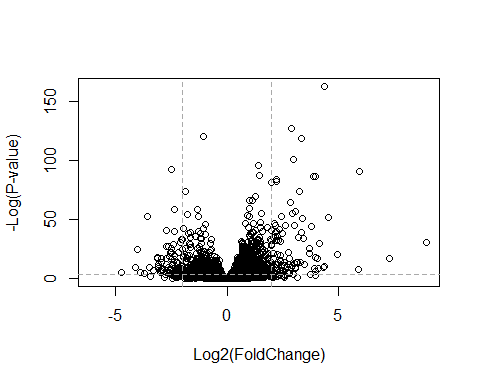
\includegraphics{class14lab_files/figure-latex/unnamed-chunk-31-1.pdf}

\begin{quote}
Q21. How do you feel about traveling for Thanksgiving and meeting for
in-person class next Week?
\end{quote}

I feel a bit uncomfortable going to in person classes, but am okay with
going if necessary.

\begin{Shaded}
\begin{Highlighting}[]
\FunctionTok{sessionInfo}\NormalTok{()}
\end{Highlighting}
\end{Shaded}

\begin{verbatim}
## R version 4.1.2 (2021-11-01)
## Platform: x86_64-w64-mingw32/x64 (64-bit)
## Running under: Windows 10 x64 (build 19043)
## 
## Matrix products: default
## 
## locale:
## [1] LC_COLLATE=English_United States.1252 
## [2] LC_CTYPE=English_United States.1252   
## [3] LC_MONETARY=English_United States.1252
## [4] LC_NUMERIC=C                          
## [5] LC_TIME=English_United States.1252    
## 
## attached base packages:
## [1] stats     graphics  grDevices utils     datasets  methods   base     
## 
## other attached packages:
## [1] ggplot2_3.3.5   dplyr_1.0.7     zipcodeR_0.3.3  lubridate_1.8.0
## [5] skimr_2.1.3    
## 
## loaded via a namespace (and not attached):
##  [1] httr_1.4.2         tidyr_1.2.0        bit64_4.0.5        jsonlite_1.7.3    
##  [5] assertthat_0.2.1   sp_1.4-6           highr_0.9          blob_1.2.2        
##  [9] yaml_2.2.1         tidycensus_1.1     pillar_1.7.0       RSQLite_2.2.9     
## [13] lattice_0.20-45    glue_1.6.0         uuid_1.0-3         digest_0.6.27     
## [17] rvest_1.0.2        colorspace_2.0-2   htmltools_0.5.1.1  pkgconfig_2.0.3   
## [21] raster_3.5-15      purrr_0.3.4        scales_1.1.1       terra_1.5-17      
## [25] tzdb_0.2.0         tigris_1.5.1       tibble_3.1.6       proxy_0.4-26      
## [29] farver_2.1.0       generics_0.1.2     ellipsis_0.3.2     withr_2.4.3       
## [33] cachem_1.0.6       repr_1.1.4         cli_3.1.1          magrittr_2.0.1    
## [37] crayon_1.4.2       memoise_2.0.1      maptools_1.1-2     evaluate_0.14     
## [41] fansi_1.0.2        xml2_1.3.3         foreign_0.8-82     class_7.3-20      
## [45] tools_4.1.2        hms_1.1.1          lifecycle_1.0.1    stringr_1.4.0     
## [49] munsell_0.5.0      compiler_4.1.2     e1071_1.7-9        rlang_0.4.11      
## [53] classInt_0.4-3     units_0.8-0        grid_4.1.2         rstudioapi_0.13   
## [57] rappdirs_0.3.3     labeling_0.4.2     base64enc_0.1-3    rmarkdown_2.11    
## [61] gtable_0.3.0       codetools_0.2-18   DBI_1.1.2          curl_4.3.2        
## [65] R6_2.5.1           knitr_1.37         rgdal_1.5-28       fastmap_1.1.0     
## [69] bit_4.0.4          utf8_1.2.2         KernSmooth_2.23-20 readr_2.1.2       
## [73] stringi_1.7.6      Rcpp_1.0.8         vctrs_0.3.8        sf_1.0-6          
## [77] tidyselect_1.1.1   xfun_0.29
\end{verbatim}

\end{document}
